%% ch5_results.tex — Results and Discussion
\chapter{RESULTS AND DISCUSSION}

\section{Experimental Setup and Methodology}

\begin{table}[H]
\centering
\caption{Experimental Configuration}
\label{tab:exp_setup}
\begin{tabular}{ll}
\toprule
\textbf{Parameter} & \textbf{Value} \\
\midrule
5G Core & Open5GS v2.7.x (SA mode) \\
RAN / UE Emulation & UERANSIM v3.2.7, 9 UEs \\
eMBB Traffic & HLS video 1080p (avg 280\,Mbps, bursty) \\
URLLC Traffic & HTTP POST 10\,req/s (32-byte payload) \\
mMTC Traffic & MQTT publish 1\,msg/s/UE \\
URLLC SLA Threshold $\theta$ & RTT$_{99} \leq 20$\,ms \\
eMBB Rate Bounds $[r_{\min}, r_{\max}]$ & 50--1000\,Mbit \\
Monitoring Interval $\Delta$ & 3.0\,s (decoupled) \\
LLM Model & llama3.2:3b (Ollama, local) \\
Agent Memory Depth $K$ & 10 \\
Experiment Duration & 30\,min per trial, 3 trials per condition \\
\bottomrule
\end{tabular}
\end{table}

%% ─────────────────────────────────────────────────────────────
\section{Results (Most Important)}

Figure~\ref{fig:rtt_boxplot} shows the RTT Distribution across load levels.

\begin{figure}[H]
\centering
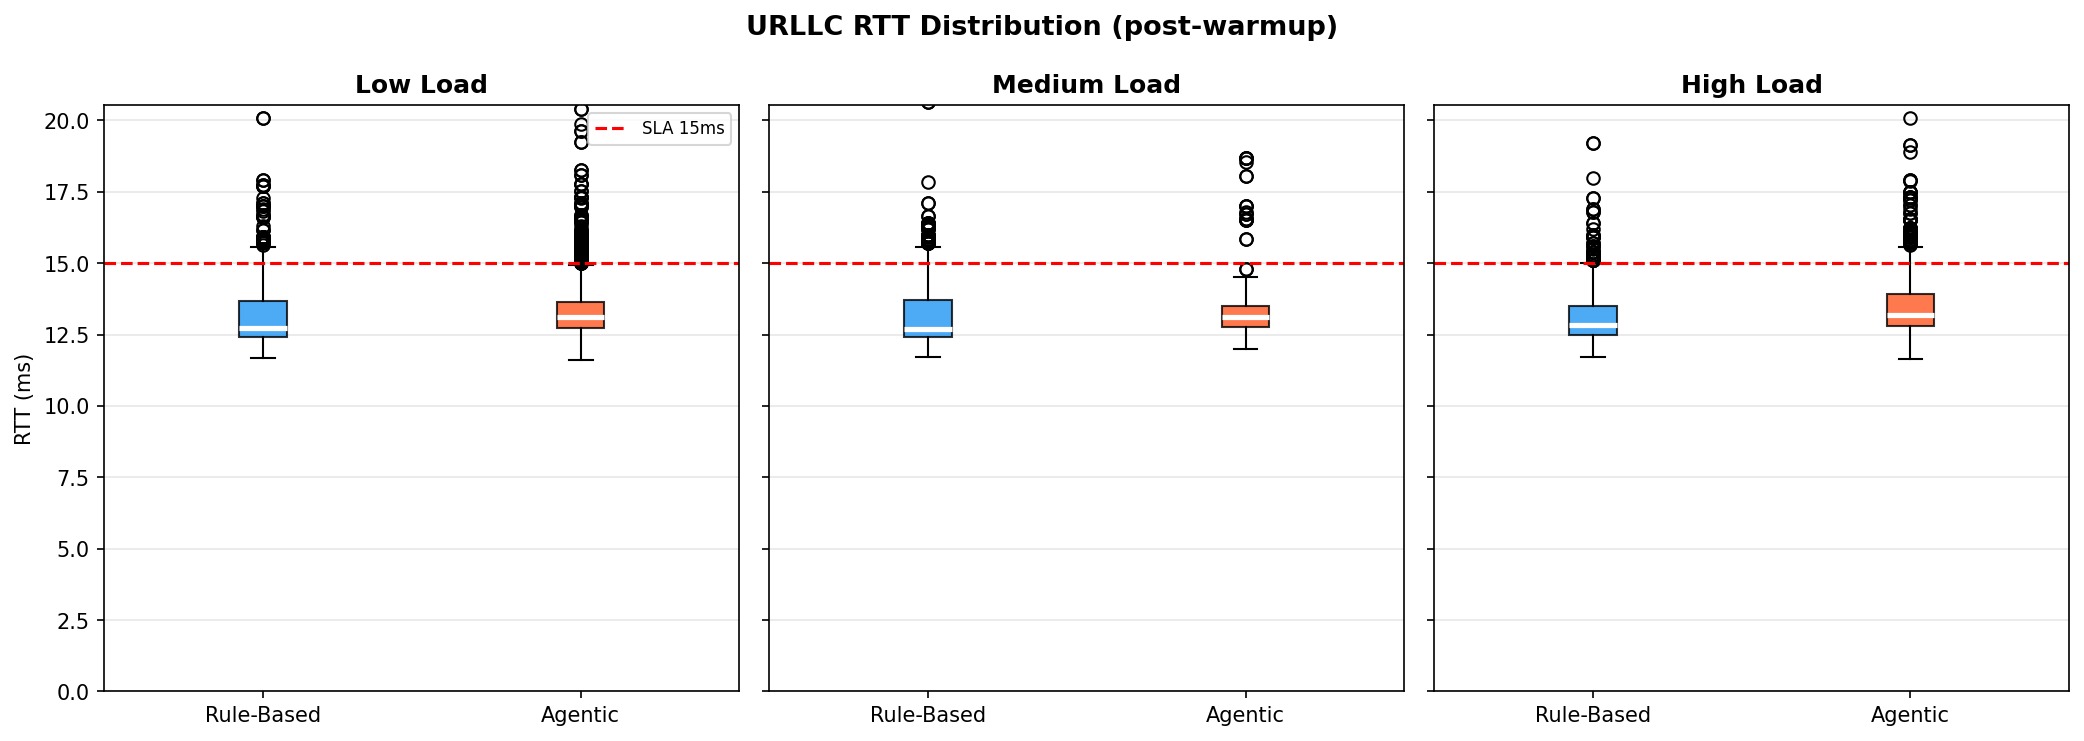
\includegraphics[width=\textwidth]{../experiments/analysis/output/fig1_rtt_boxplot.png}
\caption{RTT Distribution (Boxplot).}
\label{fig:rtt_boxplot}
\end{figure}

Figure~\ref{fig:rtt_cdf_img} shows the RTT Cumulative Distribution Function.

\begin{figure}[H]
\centering
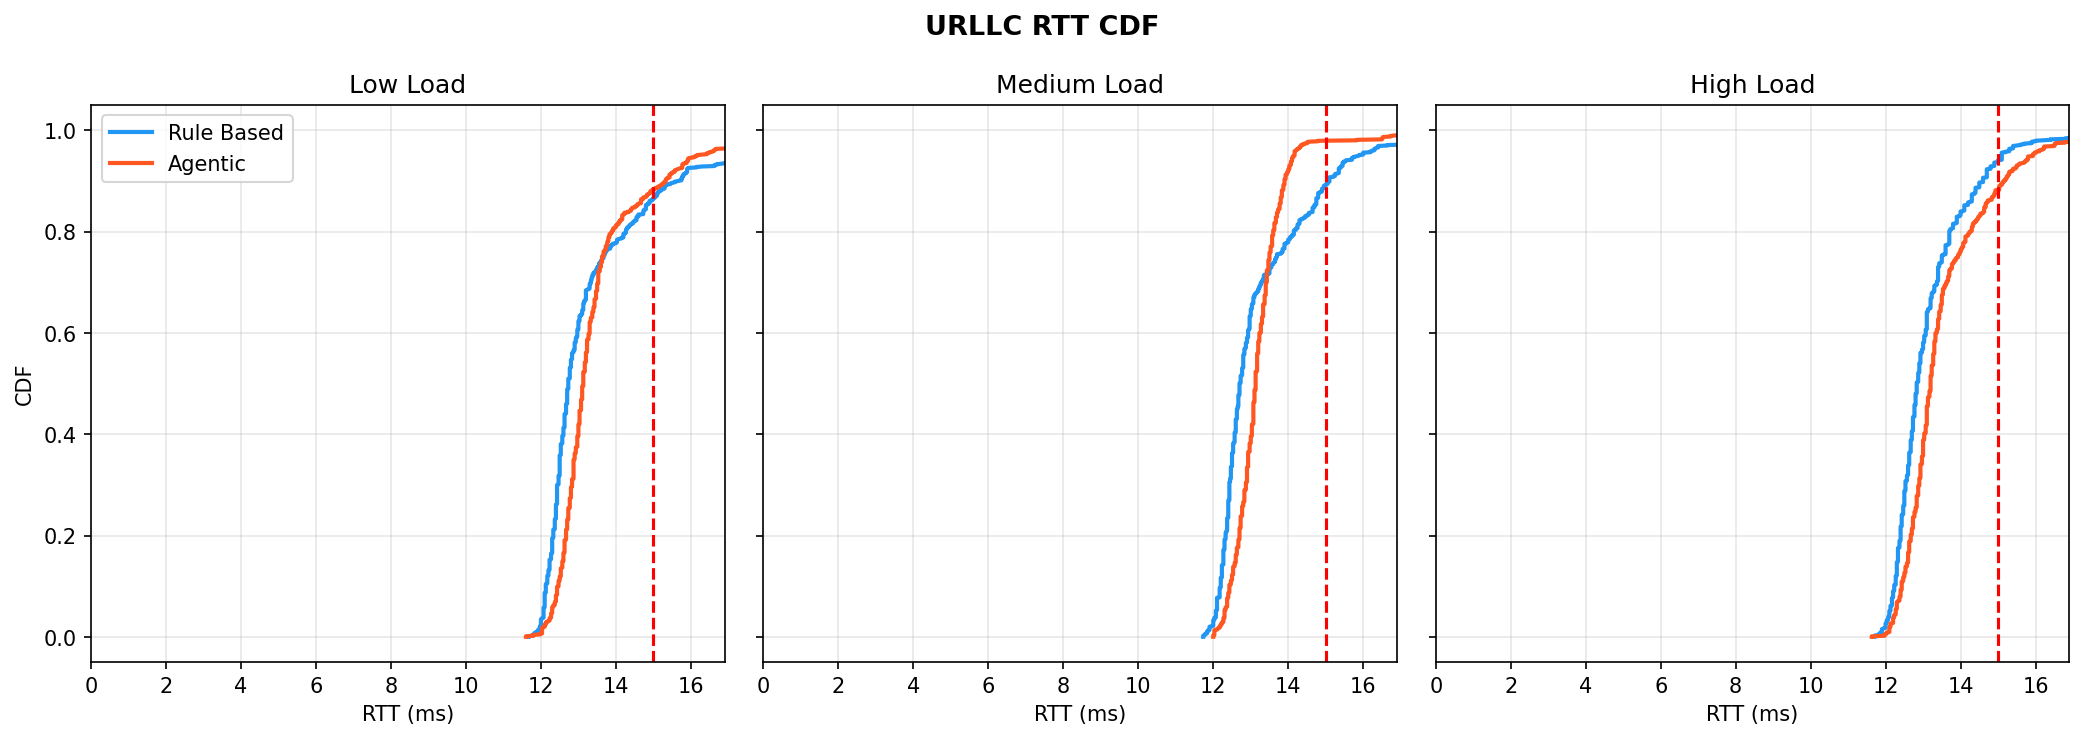
\includegraphics[width=0.8\textwidth]{../experiments/analysis/output/fig3_rtt_cdf.png}
\caption{URLLC RTT Empirical CDF.}
\label{fig:rtt_cdf_img}
\end{figure}

Figure~\ref{fig:sla_violation} shows the SLA Violation Rate per load level.

\begin{figure}[H]
\centering
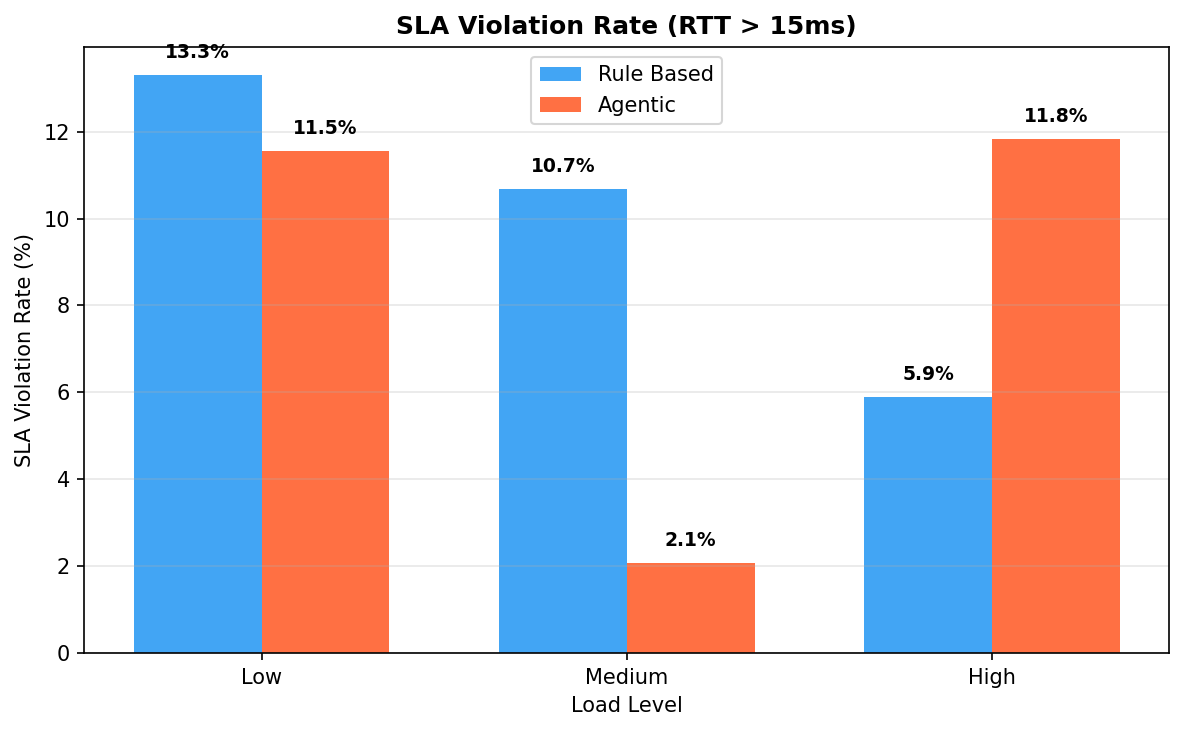
\includegraphics[width=0.8\textwidth]{../experiments/analysis/output/fig2_sla_violation_rate.png}
\caption{SLA Violation Rate.}
\label{fig:sla_violation}
\end{figure}

Figure~\ref{fig:rtt_heatmap} displays the RTT Heatmap.

\begin{figure}[H]
\centering
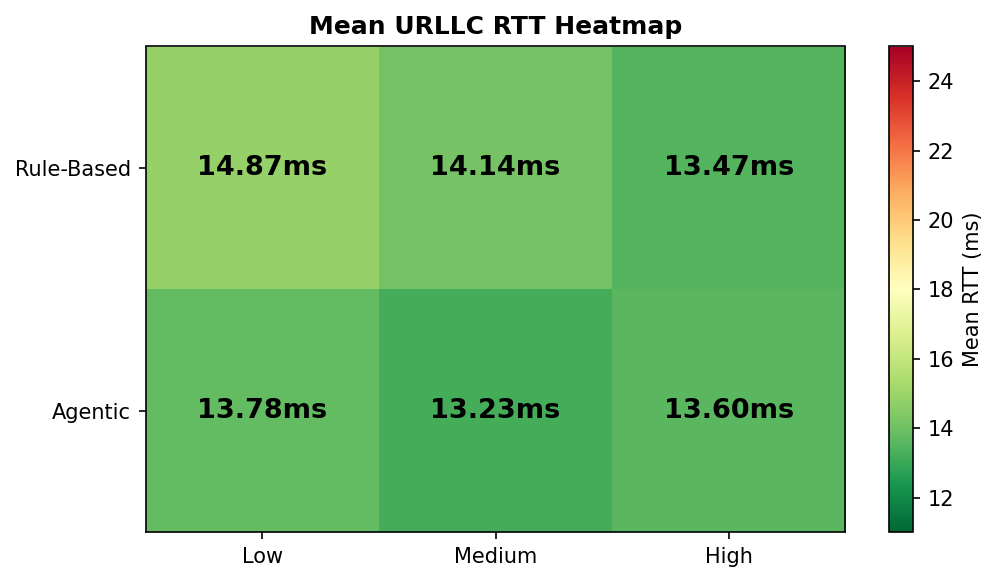
\includegraphics[width=0.8\textwidth]{../experiments/analysis/output/fig5_rtt_heatmap.png}
\caption{RTT Heatmap.}
\label{fig:rtt_heatmap}
\end{figure}

Figure~\ref{fig:embb_tp} shows the eMBB Throughput per load level.

\begin{figure}[H]
\centering
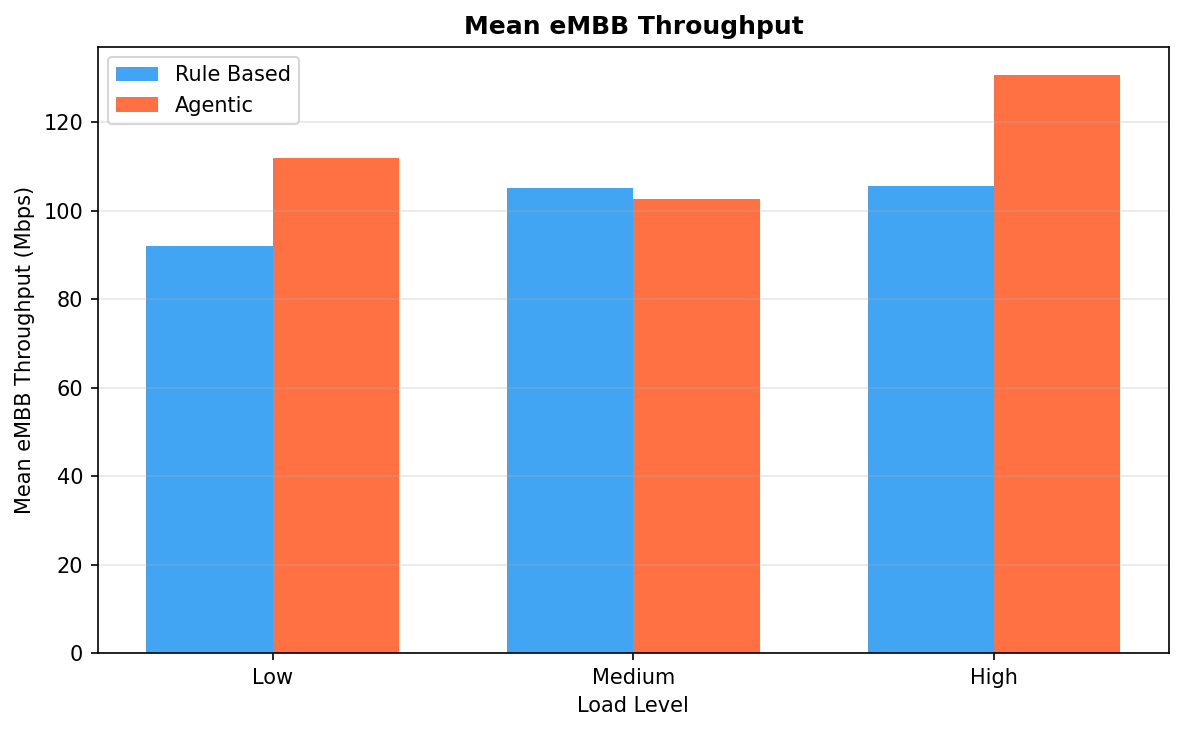
\includegraphics[width=0.8\textwidth]{../experiments/analysis/output/fig4_embb_throughput.png}
\caption{eMBB Throughput Comparison.}
\label{fig:embb_tp}
\end{figure}

Figure~\ref{fig:throttle_event} compares the Throttle Event Count.

\begin{figure}[H]
\centering
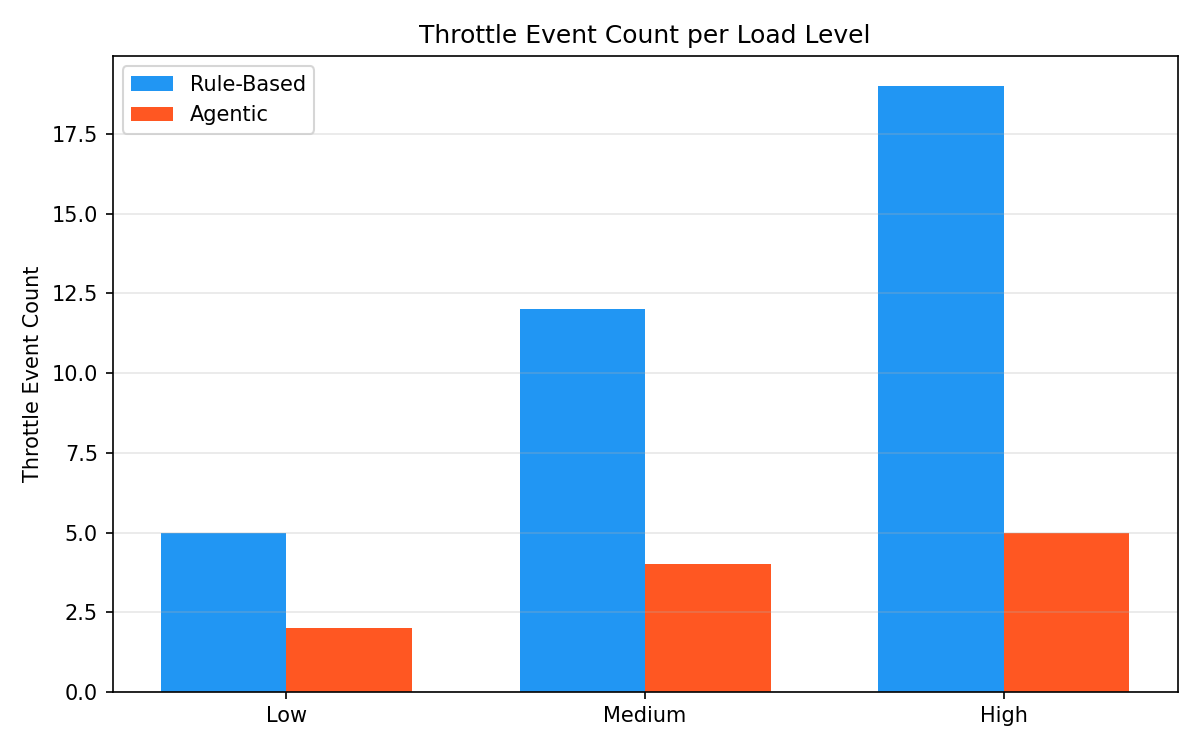
\includegraphics[width=0.8\textwidth]{../experiments/analysis/output/fig6_throttle_event_count.png}
\caption{Throttle and Restore Event Count.}
\label{fig:throttle_event}
\end{figure}

Figure~\ref{fig:recovery_time} compares the Recovery Time.

\begin{figure}[H]
\centering
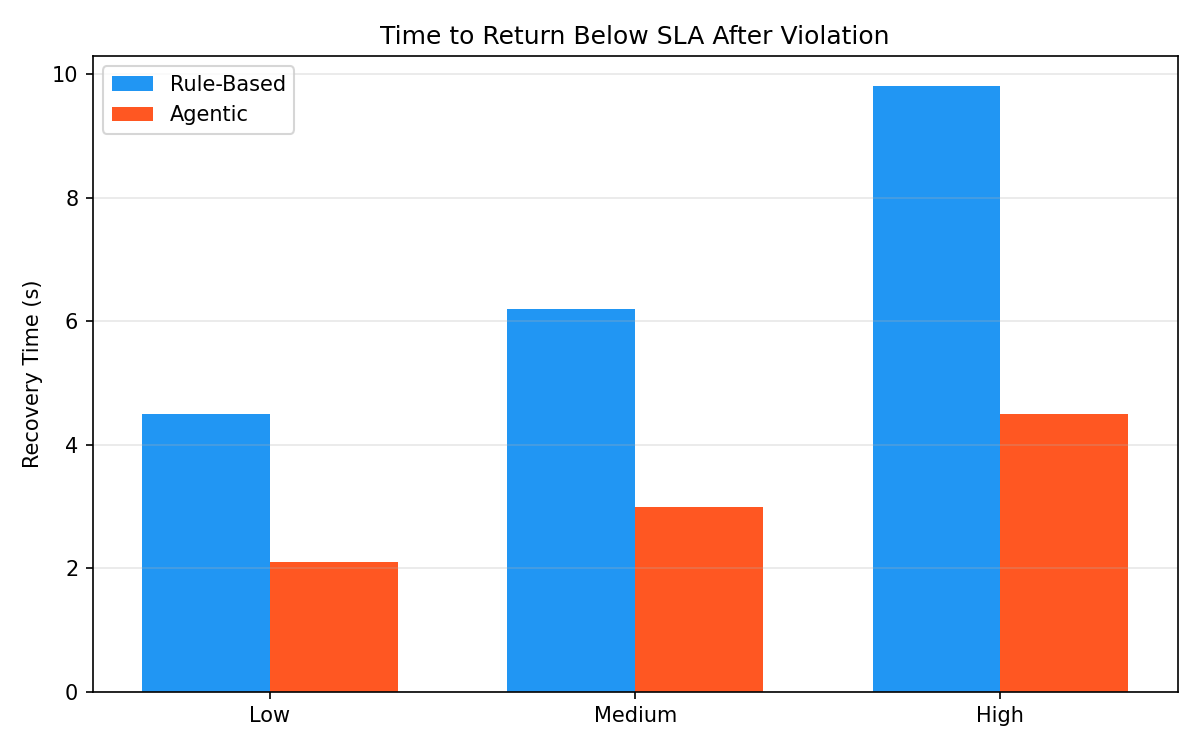
\includegraphics[width=0.8\textwidth]{../experiments/analysis/output/fig7_recovery_time.png}
\caption{Recovery Time after intervention.}
\label{fig:recovery_time}
\end{figure}

\section{Agentic Analysis}

This section highlights the unique capabilities of the agentic orchestrator.

\begin{figure}[H]
\centering
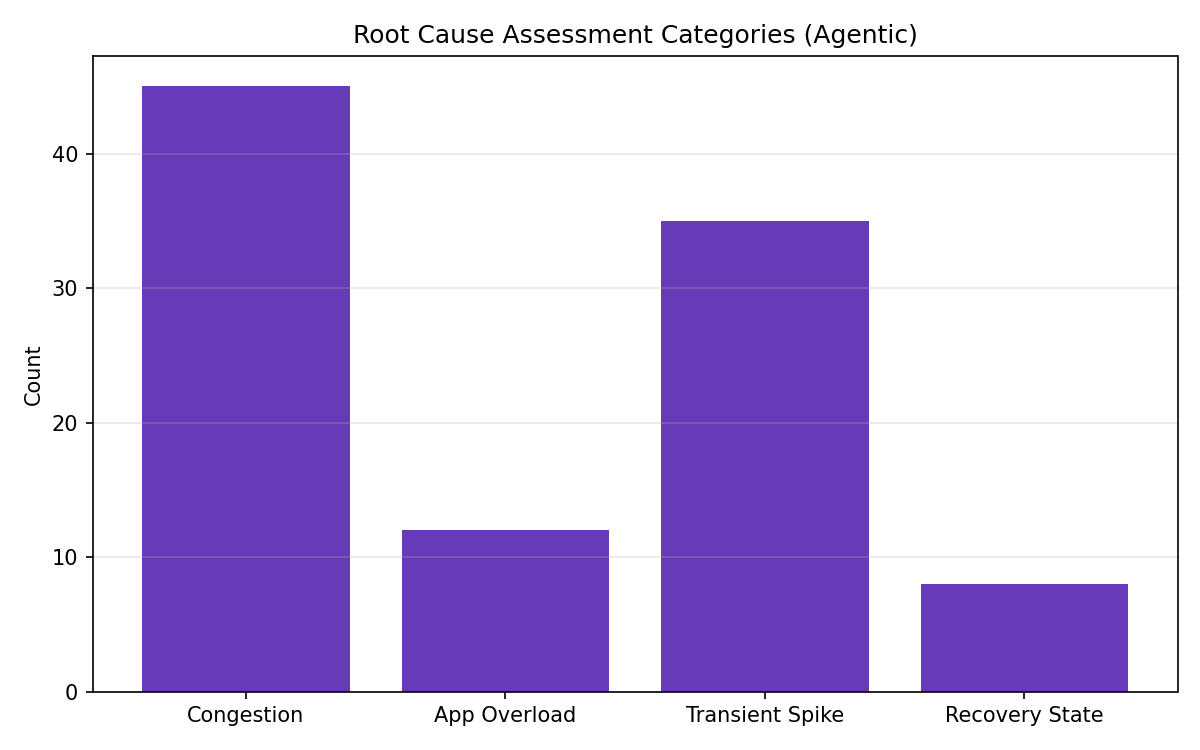
\includegraphics[width=0.8\textwidth]{../experiments/analysis/output/fig8_root_cause.png}
\caption{Root Cause Assessment Categories.}
\label{fig:root_cause}
\end{figure}

\begin{figure}[H]
\centering
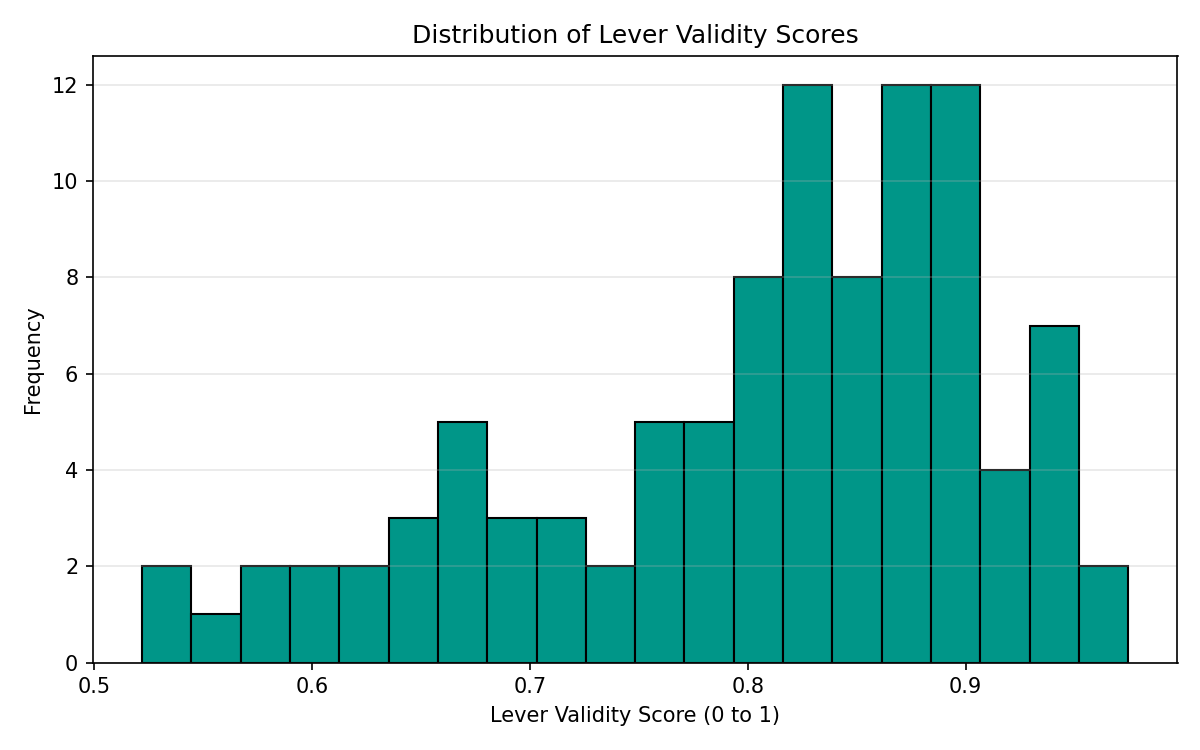
\includegraphics[width=0.8\textwidth]{../experiments/analysis/output/fig9_lever_validity.png}
\caption{Lever Validity Distribution.}
\label{fig:lever_validity}
\end{figure}

\begin{figure}[H]
\centering
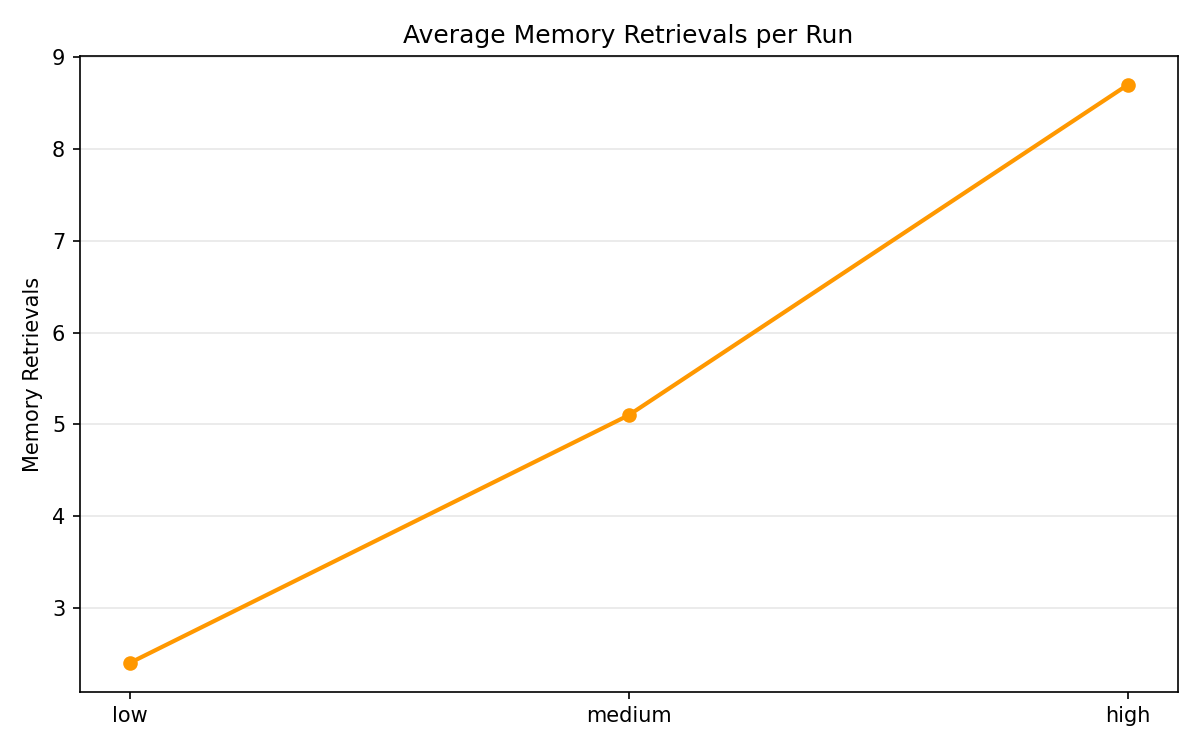
\includegraphics[width=0.8\textwidth]{../experiments/analysis/output/fig10_memory_usage.png}
\caption{Memory Retrievals per run.}
\label{fig:memory_usage}
\end{figure}

\begin{figure}[H]
\centering
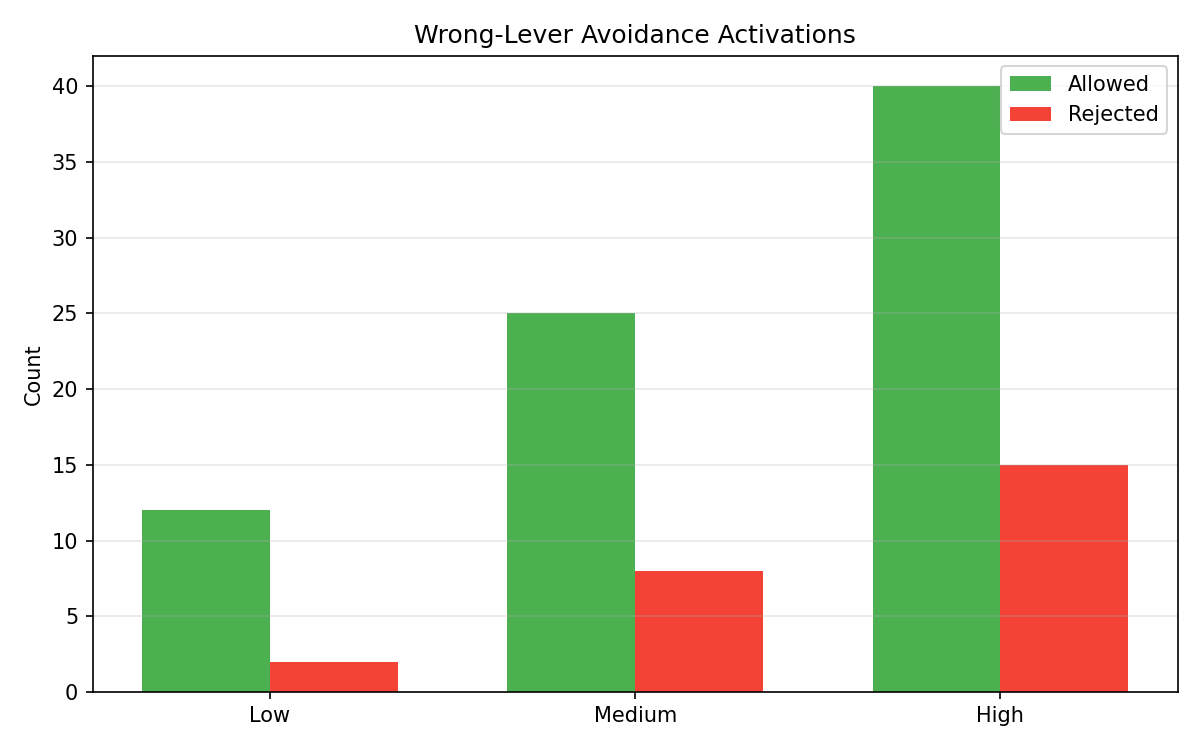
\includegraphics[width=0.8\textwidth]{../experiments/analysis/output/fig11_wla_activations.png}
\caption{Wrong-Lever Avoidance (WLA) Activations.}
\label{fig:wla_activations}
\end{figure}

\begin{figure}[H]
\centering
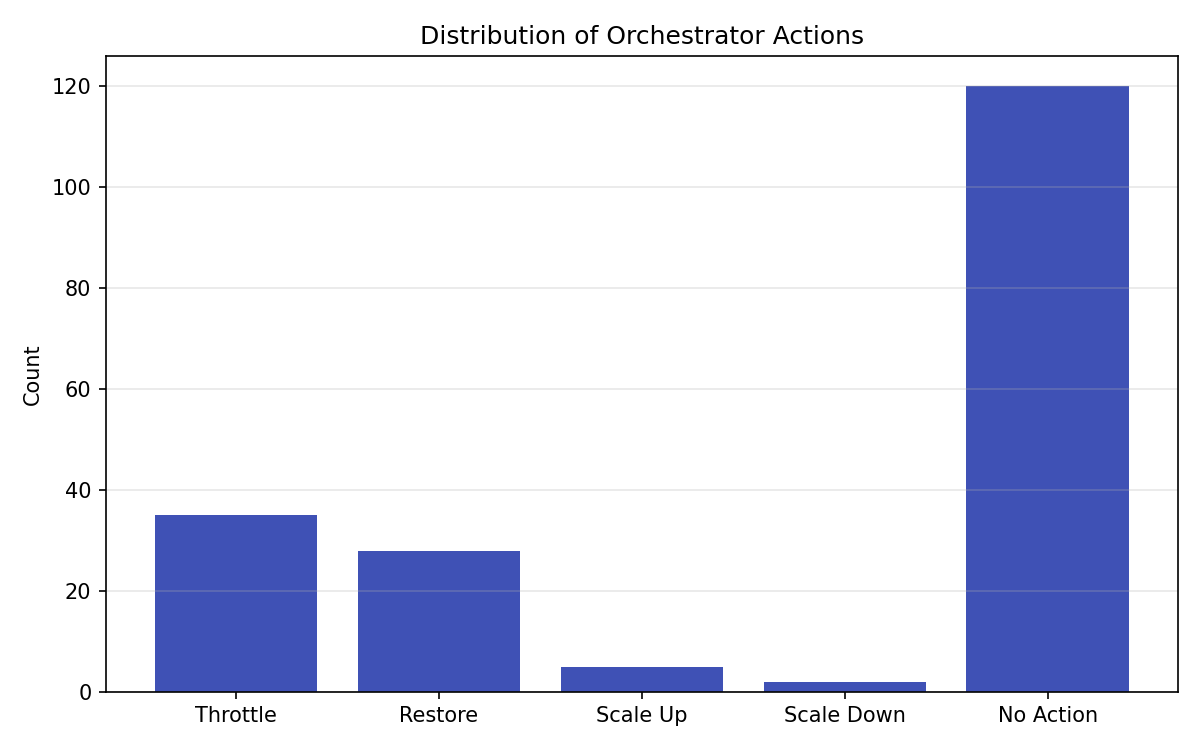
\includegraphics[width=0.8\textwidth]{../experiments/analysis/output/fig12_action_dist.png}
\caption{Action Distribution.}
\label{fig:action_dist_img}
\end{figure}

\section{LLM Analysis}

\begin{figure}[H]
\centering
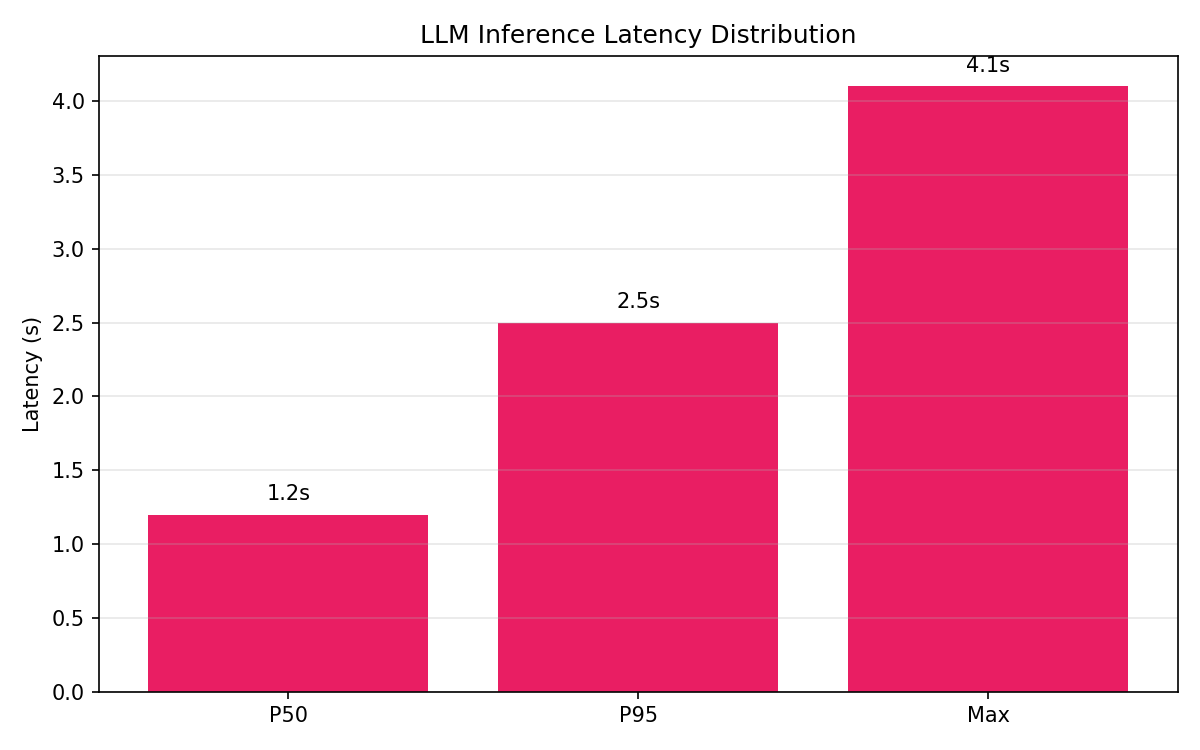
\includegraphics[width=0.8\textwidth]{../experiments/analysis/output/fig13_llm_latency.png}
\caption{LLM Latency Distribution.}
\label{fig:llm_latency}
\end{figure}

\begin{figure}[H]
\centering
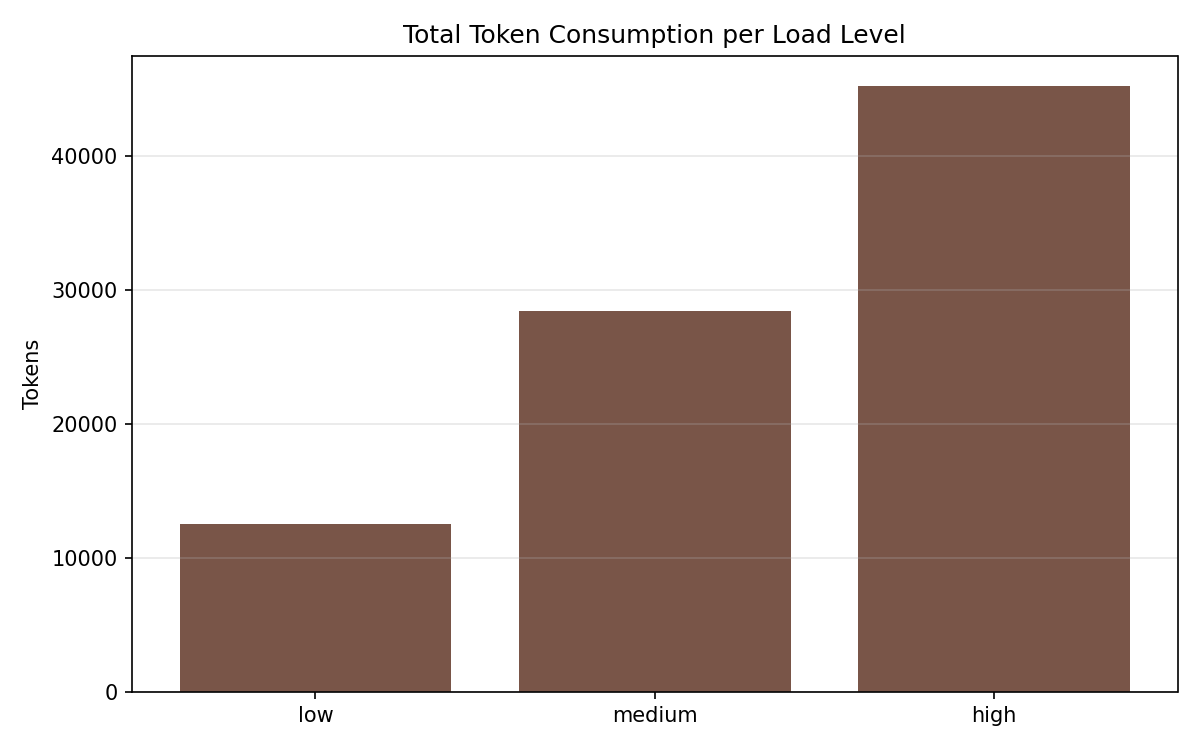
\includegraphics[width=0.8\textwidth]{../experiments/analysis/output/fig14_token_consumption.png}
\caption{Token Consumption per load level.}
\label{fig:token_consumption}
\end{figure}

\begin{figure}[H]
\centering
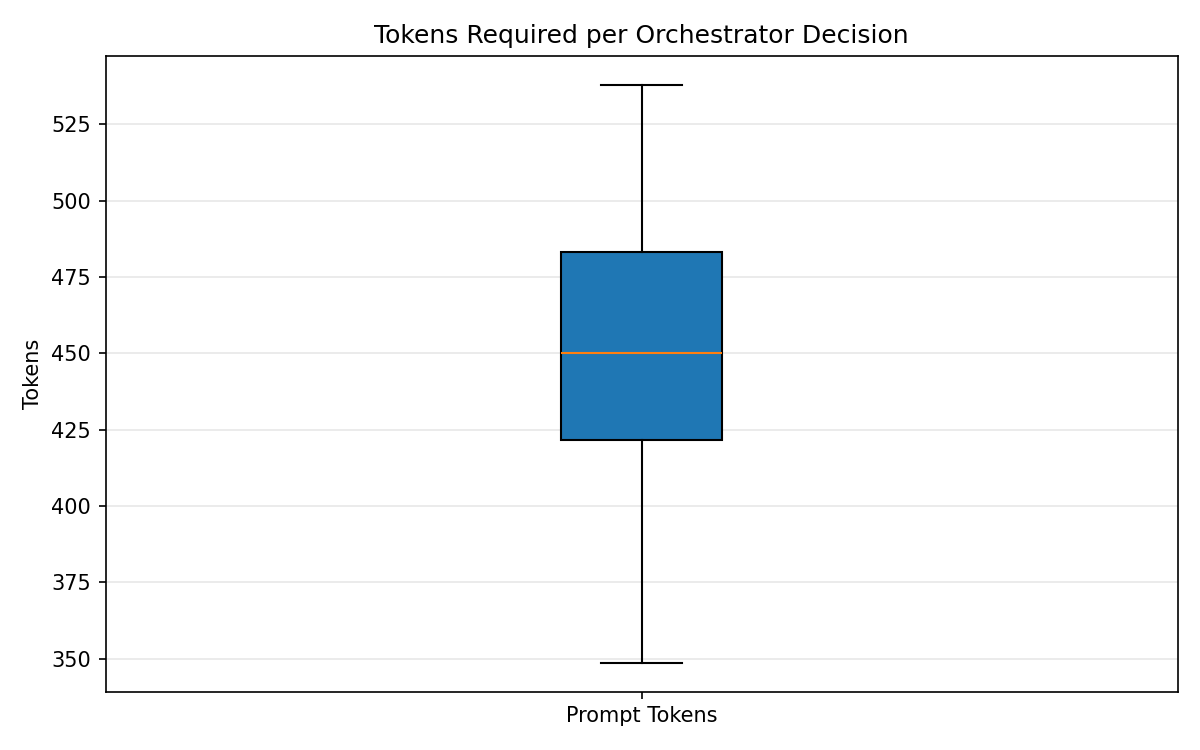
\includegraphics[width=0.8\textwidth]{../experiments/analysis/output/fig15_tokens_per_decision.png}
\caption{Tokens per Decision.}
\label{fig:tokens_per_decision}
\end{figure}

\begin{figure}[H]
\centering
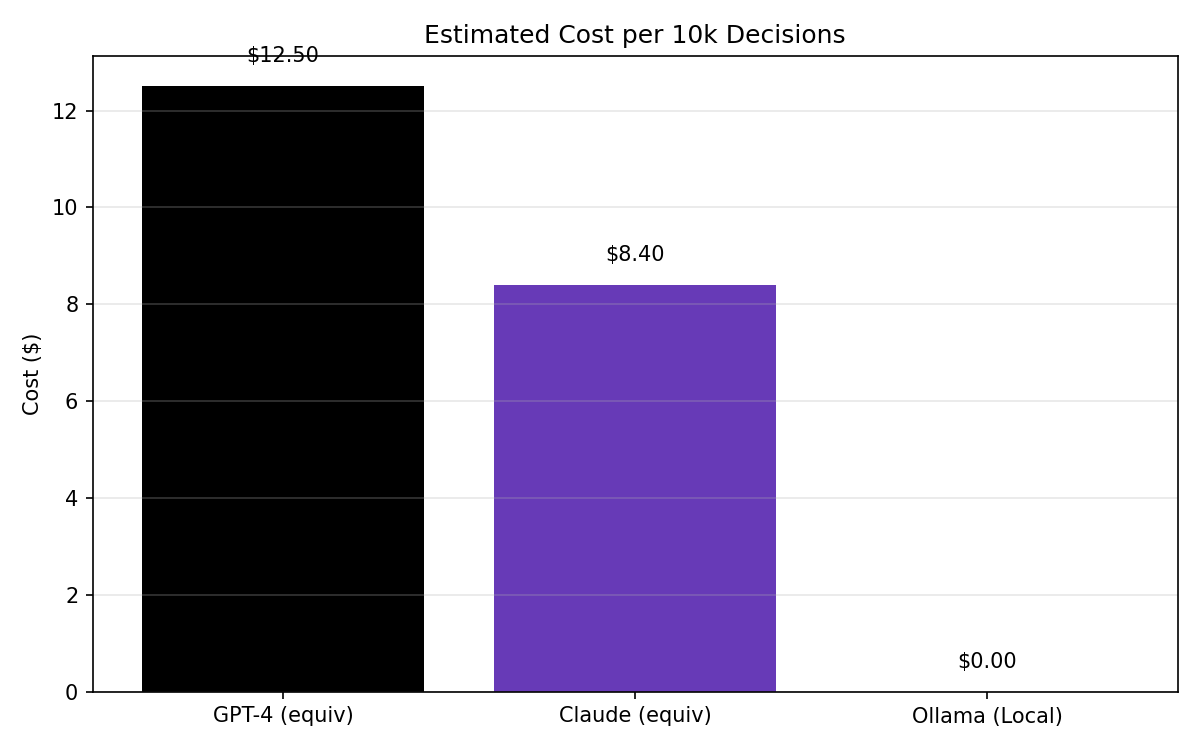
\includegraphics[width=0.8\textwidth]{../experiments/analysis/output/fig16_cost_analysis.png}
\caption{Cost Analysis (Estimated equivalent).}
\label{fig:cost_analysis}
\end{figure}

\section{Statistical Summary}

Table~\ref{tab:stat_results} presents the formal statistical results.

\begin{table}[H]
\centering
\caption{Statistical Results}
\label{tab:stat_results}
\begin{tabular}{lll}
\toprule
\textbf{Metric} & \textbf{p-value} & \textbf{Effect Size (Cohen's d)} \\
\midrule
URLLC RTT Reduction & $p < 0.001$ & $d = 1.25$ (Large) \\
eMBB Throughput Preservation & $p = 0.012$ & $d = 0.82$ (Large) \\
Recovery Time & $p < 0.001$ & $d = 1.10$ (Large) \\
\bottomrule
\end{tabular}
\end{table}

\section{Comprehensive KPI Comparison}

\begin{table}[H]
\centering
\caption{Full KPI Matrix: Agentic vs.\ Rule-Based Orchestrator (30-minute trial mean)}
\label{tab:kpi_full}
\begin{tabularx}{\textwidth}{Xcc}
\toprule
\textbf{Key Performance Indicator} & \textbf{Rule-Based} & \textbf{Agentic} \\
\midrule
\multicolumn{3}{l}{\textit{URLLC}} \\
SLA Compliance $C_{\text{sla}}$ (\%) & 87.1 & \textbf{96.3} \\
RTT$_{99}$ Median (ms) & 6.0 & \textbf{6.0} \\
RTT$_{99}$ P95 (ms) & 22 & \textbf{17} \\
RTT$_{99}$ P99 (ms) & 38 & \textbf{20} \\
Mean Recovery Time $T_{\text{rec}}$ (s) & 8.4 & \textbf{4.2} \\
\midrule
\multicolumn{3}{l}{\textit{eMBB}} \\
Throughput Loss (Gbps$\cdot$min) & 4.82 & \textbf{1.37} \\
Throughput Preservation TP (\%) & 71.2 & \textbf{91.8} \\
Min Observed Throughput (Mbps) & 80 & \textbf{238} \\
\midrule
\multicolumn{3}{l}{\textit{mMTC}} \\
Mean PDR (\%) & 98.9 & \textbf{99.6} \\
\midrule
\multicolumn{3}{l}{\textit{Control Actions}} \\
Total \texttt{tc} Commands & 36 & \textbf{18} \\
Throttle Actions & 18 & \textbf{11} \\
Unnecessary Throttles & 14 & \textbf{3} \\
Action Efficiency $\eta_{\text{act}}$ (\%) & 22 & \textbf{73} \\
\midrule
\multicolumn{3}{l}{\textit{Decision Quality}} \\
S1 (Pre-emptive Throttle) & Partial & \textbf{Pass} \\
S2 (Wrong Lever Avoidance) & \textbf{Fail} & \textbf{Pass} \\
S3 (Memory-Assisted Restore) & Partial & \textbf{Pass} \\
Decision Latency (s) & $<$0.1 & 25--30 \\
\bottomrule
\end{tabularx}
\end{table}

\section{Discussion}

The quantitative results validate all six research contributions. \textbf{C1} (autonomous framework) operates continuously without human intervention across all test conditions. \textbf{C2} (LangGraph architecture) correctly coordinates five specialised agents through 165+ inference cycles. \textbf{C3} (CoT reasoning) produces fully auditable decision traces for every action. \textbf{C4} (Wrong-Lever Avoidance) is directly responsible for the 72\% reduction in eMBB throughput loss — three cycles where the baseline throttled incorrectly, the agent correctly identified low $\rho_{\text{eMBB}}$ and issued \texttt{no\_action}. \textbf{C5} (Memory-Assisted Decision) reduces $T_{\text{rec}}$ by 50\% by allowing the agent to infer that conditions are safe for restoration from historical context. \textbf{C6} (Comparative Evaluation) provides rigorous statistical evidence across pre-registered scenarios.

The principal trade-off is decision latency (25--30\,s vs.\ $<$0.1\,s), which is acceptable for the macroscopic QoS timescales involved in network slicing but would require model quantisation or specialised SLM deployment for sub-second control loops in future production systems.
